\documentclass[11pt]{article}
\usepackage{amsmath,amssymb,amsthm}

\usepackage{url}

\usepackage{graphicx}
\graphicspath{ {./images/} }

\usepackage{multirow}

\usepackage{fixltx2e}

\DeclareMathOperator*{\E}{\mathbb{E}}
\let\Pr\relax
\DeclareMathOperator*{\Pr}{\mathbb{P}}

\newcommand{\eps}{\varepsilon}
\newcommand{\inprod}[1]{\left\langle #1 \right\rangle}
\newcommand{\R}{\mathbb{R}}

\newcommand{\handout}[5]{
  \noindent
  \begin{center}
  \framebox{
    \vbox{
      \hbox to 5.78in { {\bf EEB 109L: Introduction to Marine Science Laboratory } \hfill #2 }
      \vspace{4mm}
      \hbox to 5.78in { {\Large \hfill #5  \hfill} }
      \vspace{2mm}
      \hbox to 5.78in { {\em #3 \hfill #4} }
    }
  }
  \end{center}
  \vspace*{4mm}
}

\newcommand{\lecture}[4]{\handout{#1}{#2}{#3}{Author: #4}{#1}}

\newtheorem{theorem}{Theorem}
\newtheorem{corollary}[theorem]{Corollary}
\newtheorem{lemma}[theorem]{Lemma}
\newtheorem{observation}[theorem]{Observation}
\newtheorem{proposition}[theorem]{Proposition}
\newtheorem{definition}[theorem]{Definition}
\newtheorem{claim}[theorem]{Claim}
\newtheorem{fact}[theorem]{Fact}
\newtheorem{assumption}[theorem]{Assumption}

% 1-inch margins, from fullpage.sty by H.Partl, Version 2, Dec. 15, 1988.
\topmargin 0pt
\advance \topmargin by -\headheight
\advance \topmargin by -\headsep
\textheight 8.9in
\oddsidemargin 0pt
\evensidemargin \oddsidemargin
\marginparwidth 0.5in
\textwidth 6.5in

\parindent 0in
\parskip 1.5ex

\begin{document}

\lecture{{\bf Lab 3: Sandy Beach Zonation} --- August 31st, 2018}{Summer C 2018}{TA: Tyler McCraney}{Shawn Schwartz (UID:504570447)}

\centerline{\it{*Using the Monday (Counts, Lengths) .csv data for these analyses.*}}

\section{Assignment Part 1}
\subsection{Make a scatterplot of adult (i.e., ovigerous and non-ovigerous) and recruit sand crab counts. Fit a linear regression model to the data.}
{\it Scientific evidence:}
\begin{enumerate}
	\item ``The... model... suggests some sort of carrying capacity at undisturbed sites. In these, the probability of occurrence of compensatory mechanisms (i.e. density-dependence) might take place." (Lecari and Defeo, 1999)
	\item ``The combination between stochasticity in reproductive rates and asymmetric inter-cohort interactions (density-dependent recruitment and density-dependent survival rates) could be suggested as key processes generating large variability in sandy beach populations." (Defeo et al., 2001)
\end{enumerate}

\centerline{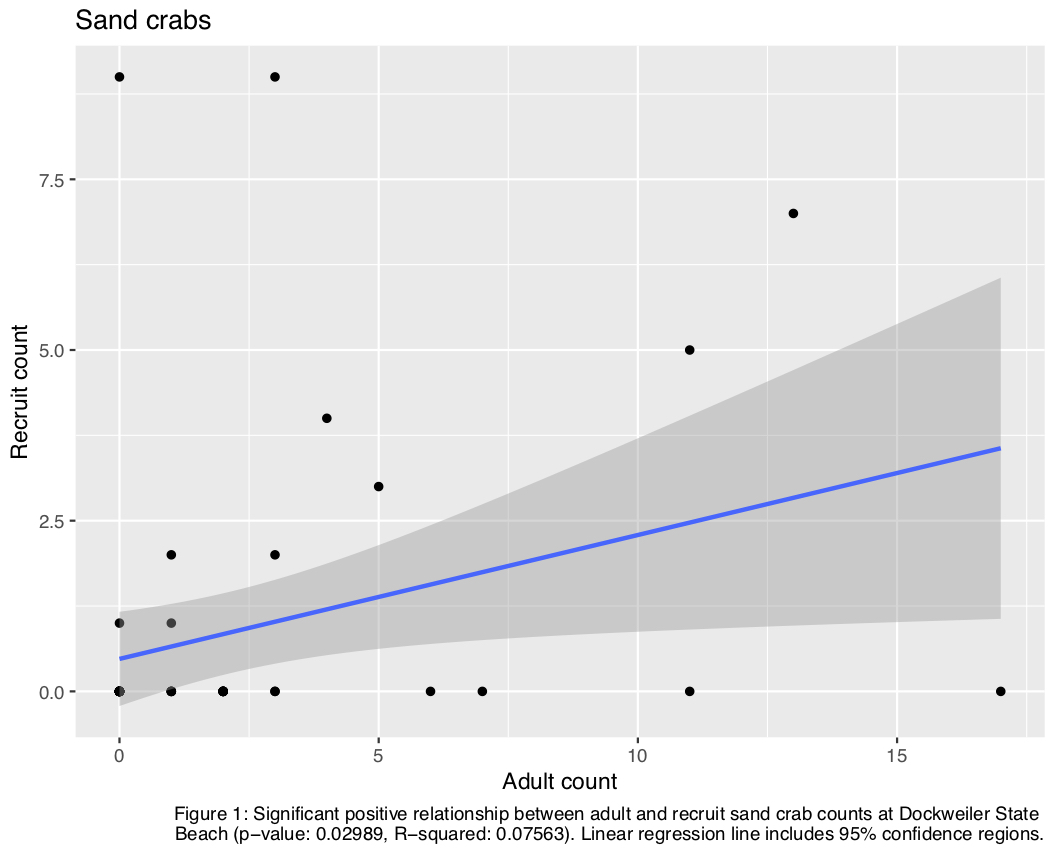
\includegraphics[scale=0.25]{Figure1}}

{\bf 1. Look at your graph. Is there a significant correlation between the two variables? If so, what is it (e.g., density-dependence), and what statistics support your finding? Is this what you expect based on the evidence above?} \\
Upon looking at the graph above, there is clearly a significant positive correlation (p-value: 0.02989) between the two variables (adult count, recruit count). The adjusted R\textsuperscript{2} value is 0.07563, which shows that although a significant positive relationship is in place, the proportion of variance of these data from the best-fit line is large, so determination of the proposed relationship should be taken skeptically. Comparing these findings to the prior literature quotes referenced above, there does seem to be a density-dependence for the recruit population relying on the proportion of adults within the sandy beach. This may be explained due to the fact that more (or less) reproductive adults would lead to more (or less) recruit offspring in the population, thus, a {\it positive} correlation as represented by these data. This is in line with the above-mentioned {\it scientific evidence}, specifically number two, in that random events in the reproductive rates of the adult and recruit sand crabs are leading to interactions supporting ``density-dependent recruitment and density-dependent survival rates" (Defeo et al., 2001). This is also in-line with Defeo et al., 2001 in that there is much variability in the sandy beach population sampled, as can be seen in the above figure. It is challenging to determine if a carrying capacity model is at play from the linear regression data above, since a polynomial logistic growth curve is needed; however, in-line with the above {\it scientific evidence}, specifically number one, there may be some sort of carrying capacity at the undisturbed sites as a consequence of the density-dependence compensatory mechanisms (Lecari and Defeo, 1999) arising from the recruitment and survival rates in variable sandy beach populations. 

\section{Assignment Part 2}
Create two size frequency histograms, one for ovigerous and one for non-ovigerous sand crab carapace lengths. Estimate the mean and 95\% confidence intervals for carapace lengths of ovigerous and non-ovigerous sand crabs.
\paragraph{}
\centerline{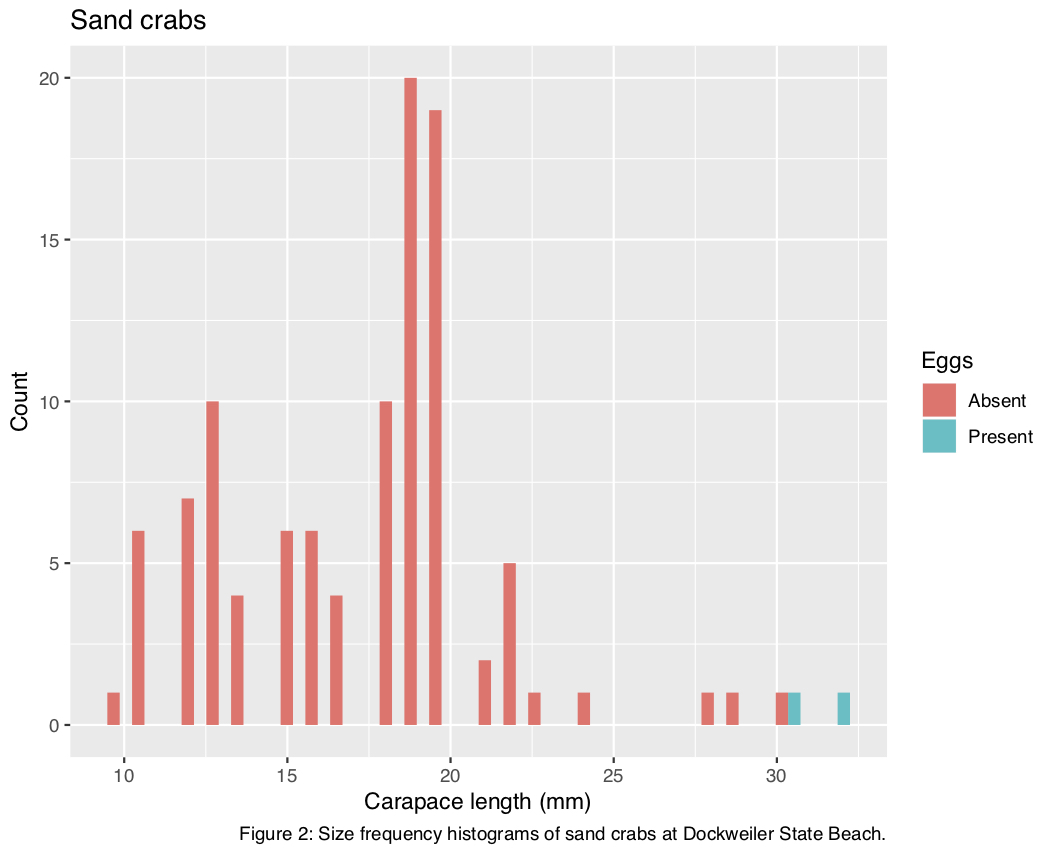
\includegraphics[scale=0.35]{Figure2}}

\subsection{Males vs Female crabs}
{\it Scientific evidence:}
\begin{enumerate}
	\item ``Female crabs obtained larger size than male crabs at all sites." Note: sampled at sites from San Diego to Humboldt County." (Dugan et al., 1994)
	\item ``Male crabs reach much smaller maximum sizes than female crabs and may have decreased survival over winter." (Dugan, 1990)
	\item ``Females of the largest modal size classes showed the highest average frequency of egg carrying and initiated egg production earliest in the season." (Cox and Dudley, 1968)
\end{enumerate}

{\bf Questions} \\
{\bf 1. Look at your histograms. How does the size of crabs with eggs compare to the size of crabs without eggs? What are the means and 95\% confidence intervals of crab lengths with eggs present and eggs absent? Is this what you expect based on the evidence above?} \\
According to the above histograms, the amount of sampled crabs with eggs present (ovigerous, blue bars) have a longer carapace length (mm) than the crabs with eggs absent (non-ovigerous, red bars). Specifically, the mean carapace length of crabs with eggs present is 31.00 mm and for crabs with eggs absent, it is 17.39 mm. The 95\% confidence intervals for crabs with eggs present is 32.96 (97.5\%) and 29.04 (2.5\%) and for crabs with eggs absent it is 18.14 (97.5\%) and 16.64 (2.5\%). In addition, the standard deviation carapace length for crabs with eggs present is 1.41 mm and for crabs with eggs absent, it is 3.91 mm. Therefore, since the 95\% confidence interval for crabs with eggs present is within one standard deviation of the carapace length means for ovigerous sand crabs, we can be confident in concluding that ovigerous sand crabs are longer in carapace length than the non-ovigerous sand crabs. As for non-ovigerous sand crabs, the 97.5\% confidence level for the 95\% confidence interval falls short of the upper-bound standard deviation. Thus, in accordance with the {\it scientific evidence} above, the current data do mostly match up to the evidence exhibited by the prior literature (Dugan et al., 1994; Dugan, 1990; Cox and Dudley, 1968) in that (1) female crabs have longer carapace lengths than male crabs, (2) male crabs are therefore maximally smaller when compared to the female crabs, and (3) the longest (and largest) female crabs had the highest average frequency of egg presence, as represented by these aforementioned data. \\

{\bf 2. How does the number of adult crabs with eggs present compare to the number of crabs without eggs? Is this what you expect based on the evidence above? Hint: Be sure to note the time of year you collected your sample.} \\
The number of adult crabs with eggs present (n = 2) compared to the number of crabs without eggs (n = 105) is indicative of there being a significantly different distribution of an abundance of adult crabs with eggs absent compared to adult crabs with eggs present. The large difference observed may be due to sampling error, but it is more likely that reproducing female sand crabs are more scarce at this time of year (later summer season). The sand crabs with eggs absent were in much greater abundance for the crabs that had a carapace length of 20 mm or less ({\it see below PivotTable}). This is expected in accordance with the {\it scientific evidence} above, specifically number three, since ``Females of the largest modal size classes showed the highest average frequency of egg carrying and initiated egg production earliest in the season" (Cox and Dudley, 1968). Although the sex of the sand crabs cannot be fully assumed, in the above histogram, for the egg-absent crabs, this may be a plausible explanation for the observed distribution of sand crabs. Since the random sampling for this study was done in the middle of the summer season (August 20th, 2018), the near 98\%:2\% distribution of assumed male:female sand crabs may be due to the expected ``tapering" effect for recruitment and thus potentially for the concurrent reproductive distribution of mating sand crabs in the later summer season months.
\paragraph{}
\centerline{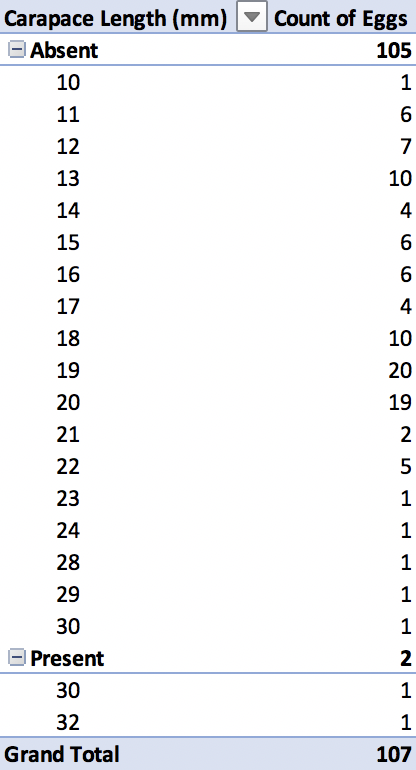
\includegraphics[scale=0.5]{PivotTable_Eggs}}

\subsection{Crab Reproduction and Recruitment}
{\it Scientific evidence:}
\begin{enumerate}
	\item ``In California, recruitment can occur from February or March through October in many years. Recruitment of this species is most intense in the spring months and tapers through the summer. A smaller late summer/fall pulse of recruitment can occur in some years in California." Note: sampled at sites from San Diego to Humboldt County. (Dugan et al., 2005)
\end{enumerate}

{\bf Questions} \\
{\bf 1. Did you find recruits in your class data? How many?} \\
Yes, in fact, out of all 149 sand crabs found during the random sampling, 43 were recruits (approximately 28.9\% of the entire sample). \\

{\bf 2. How do your class findings compare to the evidence above? Explain your answer. Hint: be sure to note the time of year that you collected your sample.} \\
Since the above {\it scientific evidence} mentions that ``recruitment can occur from February or March through October in many years. Recruitment of this species is most intense in the spring months and tapers through the summer" (Dugan et al., 2005), but our study was conducted in the later summer month of August 2018 and thus our findings seem to be in-line with the previous literature in that about 29\% of our sample were recruits in the summer, which does represent the expected ``tapering" effect of recruitment in the later summer months/season. This reasonably explains why a little over 1/4 of our sample were recruits in regard to when the sample was made (August 20th, 2018). Thus, if we would have conducted the same random sampling in November of this year, I would expect for the recruitment count to be even lower than the current amount in accordance to findings in the prior literature (Dugan et al., 2005).  



\end{document}